% chktex-file 44

\cleardoublepage%

\chapter{Resultados experimentales}%
\label{makereference7}

El sistema de optimización de baterías en el mercado eléctrico ha sido desplegado satisfactoriamente en cuatro instalaciones a lo largo de la península, tres de topología híbrida y una de topología aislada. El sistema mueve docenas de megavatios hora al día y genera millones de euros de ingresos esperados al año.

Con esto, para obtener los resultados experimentales, ha sido necesario realizar un trabajo previo de validación con el propósito de cerciorarse de los correctos resultados de las métricas operativas, es decir, investigar la rentabilidad del sistema.

Cabe destacar que, originalmente, la entidad con la que se ha realizado el despliegue del sistema apenas disponía de una herramienta rudimentaria con un funcionamiento incorrecto únicamente enfocada en el arbitraje de topología aislada. Esto significa que, precisamente debido a la novedad de los \glspl{bess}, no es posible realizar comparaciones con soluciones similares debido a su nula existencia dentro de la entidad energética misma.

Aún así, se ha estudiado el rendimiento obtenido por el sistema, analizando su uso no solo a lo largo del periodo de despliegue, sino realizando también simulaciones con datos de mercado y señales de la batería reales. Precisamente, facilitar el llamado \textit{backtesting} resulta ser una de las razones principales para el diseño de la arquitectura del sistema modular, con el \gls{pis} de la infraestructura operacional y el \gls{dw} del entorno de mercado.

De esta forma, la métrica principal a analizar resulta siempre ser el beneficio obtenido en euros megavatio hora. La razón del uso de un beneficio dependiente de la energía es el hecho de que no querer necesariamente vender la mayor cantidad disponible en todo momento, generando grandes ingresos puntuales pero perdiendo la capacidad de aumentarlos en un futuro. Lo que se busca, en cambio, es el \textit{spread}, siendo la diferencia entre el precio al que se ha vendido y comprado una unidad de energía.

\section{Rentabilidad}%
\label{makereference7.1}

En primer lugar, es necesario conocer la información de costes para determinar si verdaderamente merece la pena la incorporación de \glspl{bess} en la red eléctrica, más allá de sus beneficios operativos.

Un arquetipo de batería dimensionada en \SI{20}{\mega\watt\hour} \( E_{n} \), \SI{5}{\mega\watt} \( P_{n} \), 90 \% de eficiencia \( \eta \), 2 \% de degradación anual \( \delta \), una vida útil de 30 años \( H \) y 1 ciclo por día \( N \), suponiendo un \textit{spread} \( S \) estándar de \SI{60}{\text{\euro}\per\mega\watt\hour}, genera \SI{8\,958\,504}{\text{\euro}} de ingreso \( \pi \), según la ecuación~\ref{eq:beneficio-total}.

\begin{equation}%
  \label{eq:beneficio-total}
  \pi = \eta \cdot S \cdot E_{n} \cdot N \cdot D \cdot \frac{1 - {(1 - \delta)}^{H}}{\delta}
\end{equation}

Con ello, se debe analizar el \gls{capex} inicial y el \gls{opex} continuado de un \gls{bess} estándar de ion-litio. Precisamente, a partir de los datos de la evolución de precio de los \glspl{bess} de la figura~\ref{fig:precio-bateria}, se estima el \gls{capex} en la figura~\ref{fig:capex-bateria}. El \gls{opex} es comúnmente fijado en el 3 \% del \gls{capex}. Además, se deben tener en cuenta las ayudas del estado a las baterías, las cuales pueden cubrir hasta el 45--65 \% del coste total de la batería~\cite{solfy2025subvenciones} en la actualidad.

\begin{figure}
  \centering
  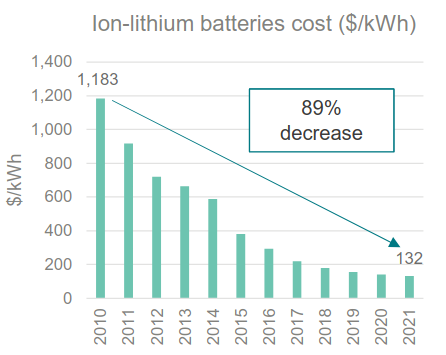
\includegraphics[width=0.5\linewidth]{figures/precio-bateria.png}
  \caption[Evolución del precio de las baterías a lo largo de los años.]{Evolución del precio de las baterías a lo largo de los años~\cite{bnef2025strategic}.}%
  \label{fig:precio-bateria}
\end{figure}

\begin{figure}
  \centering
  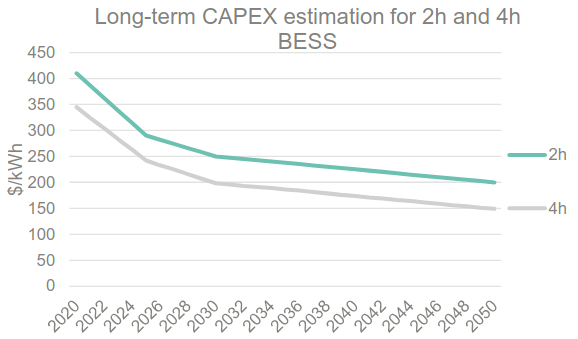
\includegraphics[width=0.5\linewidth]{figures/capex-bateria.png}
  \caption[Estimación de la evolución de los gastos de capital.]{Estimación de la evolución de los gastos de capital~\cite{national2025nrel} para baterías de 2 y 4 horas, dependiendo de su capacidad de almacenamiento entre potencia. Las baterías de 4 horas son las generalmente usadas en el arbitraje en los mercados spot.}%
  \label{fig:capex-bateria}
\end{figure}

De esta forma, con la batería a analizar y tomando el \gls{capex} como \SI{3\,842\,000}{\text{\euro}} y reducido a \SI{1\,921\,000}{\text{\euro}} por las ayudas, el \gls{opex} anual resulta en \SI{115\,260}{\text{\euro}} y \SI{57\,630}{\text{\euro}}, respectivamente\footnote{Convertido de dolares a euros.}. A lo largo de la vida útil de la batería, el coste suma \SI{7\,299\,800}{\text{\euro}} y \SI{5\,570\,900}{\text{\euro}} con ayudas.

Los resultados obtenidos indican, al igual que lo hacen autoridades pertinentes~\cite{gadvisory2025technical}, que resulta complicado rentabilizar las baterías únicamente a través la participación en los mercados spot. En la actualidad, como las ayudas a los \glspl{bess} son prominentes, las baterías gozan de una más que favorable situación de mercado de cara al futuro, en cambio, es conveniente que los sistemas de optimización de baterías en el mercado eléctrico incorporen estrategias de \textit{revenue stacking} y también oferten disponibilidades en los mercados de regulación.

\section{Operación manual}%
\label{makereference7.2}

Pruebas empíricas con participación de agentes de mercado en diversas instalaciones indican un enorme aumento de la eficiencia de optimización de la solución automatizada.

Agentes de mercado subrayan tener que realizar sesiones de dos horas diarias con el único propósito de introducir las posiciones de mercado manualmente y comunicárselas a los operadores de telecomunicaciones para mandar las consignas\footnote{Aunque no se cuente con el flujo desarrollado del sistema en el que las señales son comunicadas al \gls{pis}, existe un flujo alternativo a través de SCADA para operaciones manuales, como ya se ha descrito anteriormente.}. Este trabajo de consignación manual es extremadamente propenso a errores y completa o difícilmente incapaz de aprovechar la totalidad del proceso de optimización, debido a la cantidad de combinaciones exponenciales de las posiciones de mercado, cuanto mayor es el horizonte de optimización.

La comparativa entre los resultados manuales contra el proceso del sistema desarrollado favorecen el uso de un sistema automatizado que no solo mejore de forma directa las ganancias generadas, sino que tenga en cuenta el entorno al completo y modifique su comportamiento según el mismo.

De esta forma, sin la disposición del sistema, la estrategia de arbitraje más extendida entre los agentes de mercado es la compra y venta directa de energía en los periodos valle y pico, respectivamente. Debido a la alta complejidad del arbitraje en los mercados intradiarios, los agentes de mercado únicamente definen la posición para el mercado diario, el de mayor liquidez.

Como se puede observar en la situación de mercado\footnote{Batería híbrida de \SI{5}{{\mega\watt\hour}} de capacidad, \SI{5}{{\mega\watt}} de potencia y 100 \% de eficiencia.}, con precio de la figura~r\ref{fig:manual-auto-precio} y posición de la figura~\ref{fig:manual-auto-posicion}, los dos principales problemas de la estrategia manual son el nulo aprovechamiento de los recursos híbridos de generación en las instalaciones que lo soportan, ya que no es posible tener en cuenta las actualizaciones de las previsiones, y la generación de desvíos ante falta de casaciones en el mercado diario, que resultan en un perdida monetaria comparativamente significativa.

\begin{figure}
  \centering
  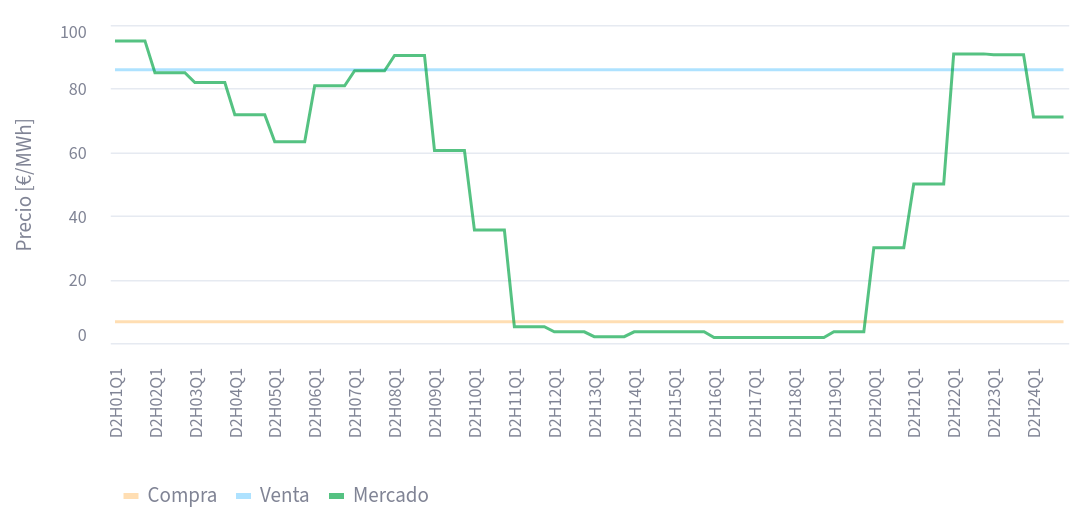
\includegraphics[width=0.75\linewidth]{figures/manual-auto-precio.png}
  \caption[Precio de mercado de la situación de operación manual.]{Precio de mercado de la situación de operación manual.}%
  \label{fig:manual-auto-precio}
\end{figure}

\begin{figure}
  \centering
  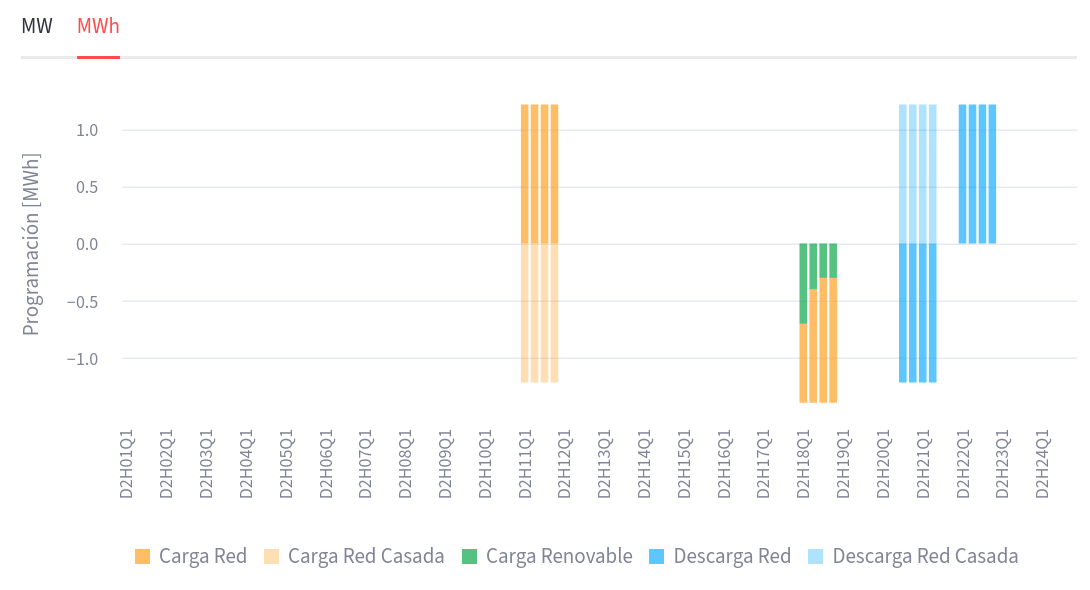
\includegraphics[width=0.75\linewidth]{figures/manual-auto-posicion.png}
  \caption[Comparación del arbitraje entre la estrategia manual y la automática.]{Comparación del arbitraje entre la estrategia manual y la empleada por el sistema. La estrategia manual se corresponde con la posición casada y la automática con la actual.}%
  \label{fig:manual-auto-posicion}
\end{figure}

Los resultados muestran como, en este caso, el arbitraje manual no es capaz de captar las variaciones de precio en los mercados intradiarios e intradiario continuo. Determinar periodos incorrectos de valle y pico, si no se disponen de estrategias de resolución de desvíos como las que aporta el sistema desarrollado, causan perdidas de \( (\SI{90.92}{\text{\euro}\per\mega\watt\hour} \cdot \SI{5}{{\mega\watt\hour}} - \SI{1.72}{\text{\euro}\per\mega\watt\hour} \cdot \SI{3.7}{{\mega\watt\hour}} ) - (\SI{50.00}{\text{\euro}\per\mega\watt\hour} \cdot \SI{5}{{\mega\watt\hour}} - \SI{6.72}{\text{\euro}\per\mega\watt\hour} \cdot \SI{5}{{\mega\watt\hour}}) = \SI{233.04}{\text{\euro}} \) para un ciclo de la batería.

\section{Configuración topológica}%
\label{makereference7.3}

Se han realizado análisis comparativos entre el rendimiento generado por cada una de las topologías, tanto aislada como híbrida, para determinar el aumento de los ingresos que sistemas de optimización de baterías en el mercado eléctrico pueden aportar, dependiendo de la configuración de la red.

Se detalla el resultado de la posición aislada de la situación de mercado empleada en la figura~\ref{fig:posicion-aislada}, y las diferencias de beneficio comparativas en la tabla~\ref{tab:comparacion-aislada-hibrida} a favor de la topologías híbrida (analizada en su configuración más permisiva en la posterior sección~\ref{makereference7.4}), siendo capaz de enrutar los flujos de carga desde diferentes fuentes. De esta forma, es entendible la tendencia de la industria de aumentar el número de instalaciones de colocación híbridas renovables y de almacenamiento simultáneamente, a diferencia del uso de las topologías aisladas\footnote{Batería aislada de \SI{5}{{\mega\watt\hour}} de capacidad, \SI{5.25}{{\mega\watt}} de potencia y 87 \% de eficiencia.}.

La razón de la menor rentabilidad de la topología aislada viene dada porque su contraparte híbrida es capaz de cargar la batería en muchas ocasiones por precios nulos, mientras que la aislada siempre tiene que pagar por pasar por la red.

\begin{figure}
  \centering
  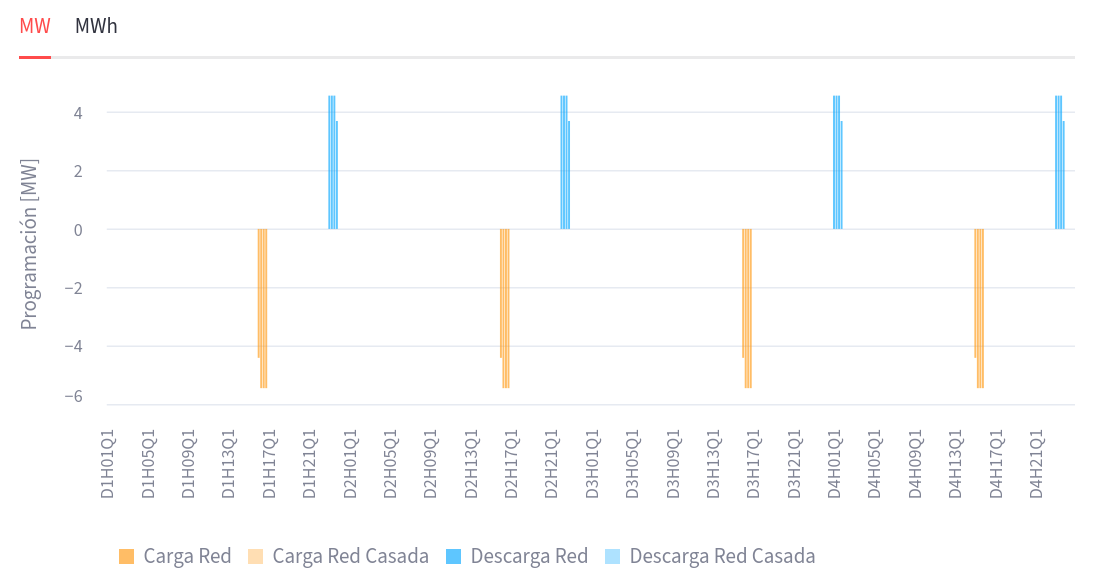
\includegraphics[width=0.5\linewidth]{figures/posicion-aislada.png}
  \caption[Resultados de arbitraje de la topología aislada.]{Resultados de arbitraje de la topología aislada.}%
  \label{fig:posicion-aislada}
\end{figure}

\begin{table}[ht]
  \centering
  \begin{tabular}{|l|S|S|S|}
    \hline
    Topología        & {Beneficio [\si{\text{\euro}\per\mega\watt\hour}]} & {Beneficio [\si{\text{\euro}}]} & Ciclos \\
    \hline
    Aislada          &  90.50                                             & 1574.40                         & 4.0    \\
    Híbrida flexible & 142.30                                             & 9562.90                         & 4.0    \\
    \hline
  \end{tabular}
  \caption[Comparación de configuraciones topológicas.]{Comparación de las métricas de las configuraciones topológicas aislada e híbrida, en donde se observa el rendimiento superior de la colocación de baterías.}%
  \label{tab:comparacion-aislada-hibrida}
\end{table}

Aún así, es importante mencionar que, aunque sea un hecho que las topologías aisladas no sean las más rentables, es posible usarlas para los mercados de disponibilidad, que están experimentando actualmente picos altísimos nunca antes vistos. Con ello, aunque sea posible obtener beneficios desorbitados regulando disponibilidades con una topología aislada (o híbrida), la incorporación de un mayor número de baterías en la red está causando la saturación del mercado de regulación, visualizada en la figura~\ref{fig:fcr-price}. Por lo tanto, resulta recomendable invertir en hibridaciones, ya que las topologías aisladas continúan perdiendo valor con el paso del tiempo. De este modo, ``aunque los mercados de ajuste todavía ofrezcan picos ocasionales que vale la pena aprovechar, las configuraciones aisladas ya no son suficientes como estrategia independiente''~\cite{leal2025case}.

\begin{figure}
  \centering
  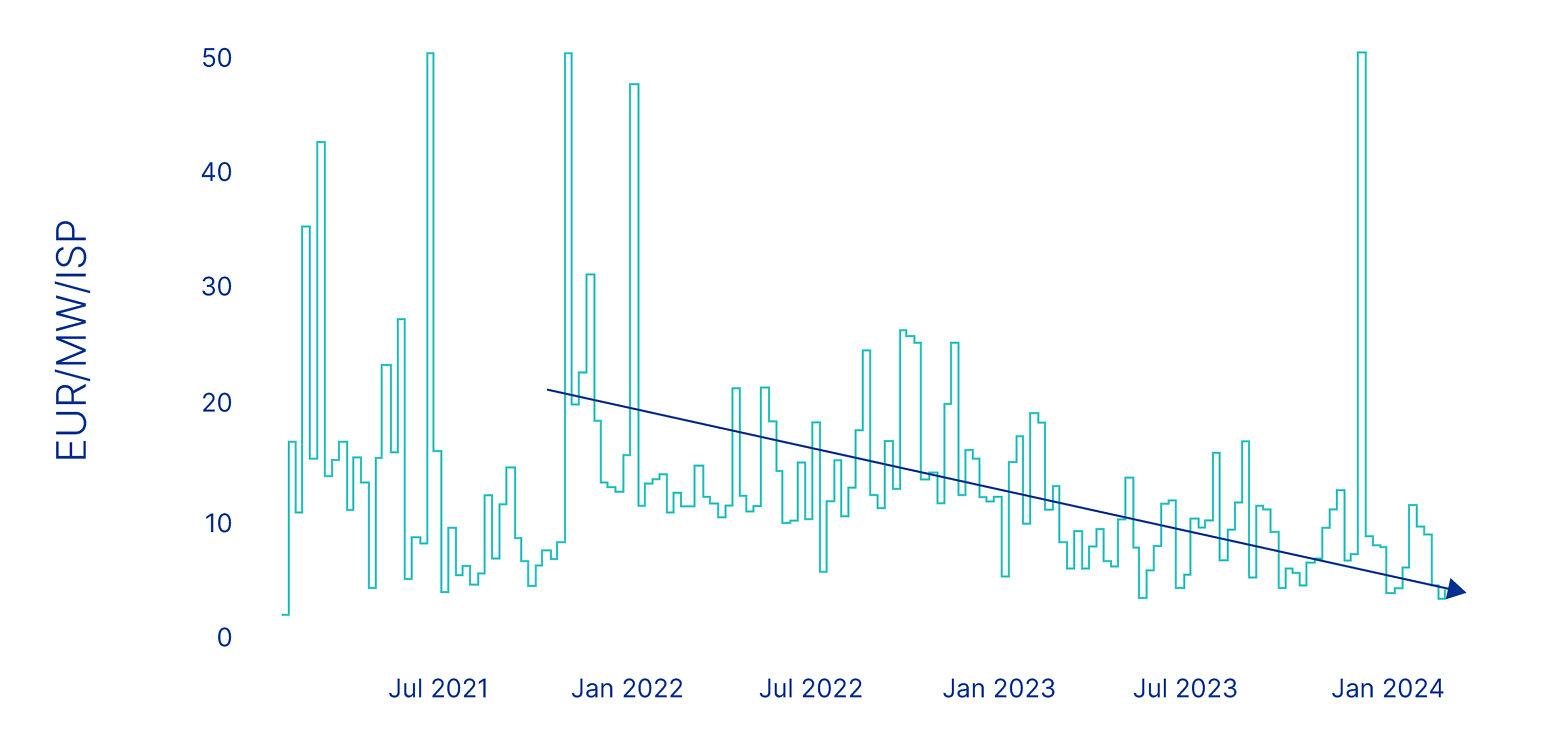
\includegraphics[width=0.75\linewidth]{figures/fcr-price.jpg}
  \caption[Descenso promedio del precio de los mercados de ajuste por periodo.]{Descenso promedio del precio de los mercados de ajuste por periodo~\cite{leal2025case}.}%
  \label{fig:fcr-price}
\end{figure}

\section{Topología híbrida}%
\label{makereference7.4}

Una vez comprobada la mejora del uso de instalaciones de topología híbrida, resulta interesante desglosar su operación en los tres modos de operación principales observados en la practica, el híbrido flexible, el híbrido con prioridad de carga de generación y el híbrido con carga aislada de la red.

Aunque las tres configuraciones híbridas sean capaces de aprovechar y rentabilizar la energía generada, es interesante comprobar cual de ellas es capaz de generar la mayor rentabilidad en una situación de mercado mostrada en la figura~\ref{fig:precios-hibridaciones}, con el propósito de priorizar su instalación.

\begin{figure}
  \centering
  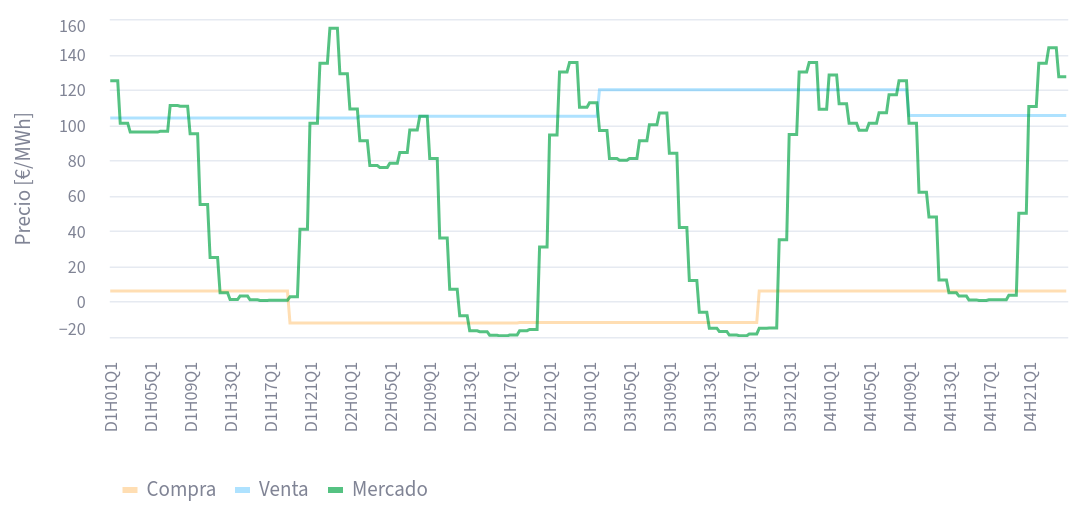
\includegraphics[width=0.75\linewidth]{figures/precios-hibridaciones.png}
  \caption[Precios de la situación de mercado de la comparación de hibridaciones.]{Precios de la situación de mercado de la comparación de hibridaciones.}%
  \label{fig:precios-hibridaciones}
\end{figure}

La figura~\ref{fig:hibrida-flexible} muestra la posición de mercado de la situación analizada de la configuración híbrida flexible\footnote{Batería híbrida de \SI{20}{{\mega\watt\hour}} de capacidad, \SI{5}{{\mega\watt}} de potencia y 86 \% de eficiencia.}, en comparación con la híbrida con prioridad de carga de generación\footnote{Batería híbrida de \SI{5}{{\mega\watt\hour}} de capacidad, \SI{5}{{\mega\watt}} de potencia y 90 \% de eficiencia.} de la figura~\ref{fig:hibrida-prioridad} y la híbrida con carga aislada de la red\footnote{Batería híbrida de \SI{9.20}{{\mega\watt\hour}} de capacidad, \SI{3}{{\mega\watt}} de potencia y 90 \% de eficiencia.} de la figura~\ref{fig:hibrida-aislada}.

\begin{figure}
  \centering
  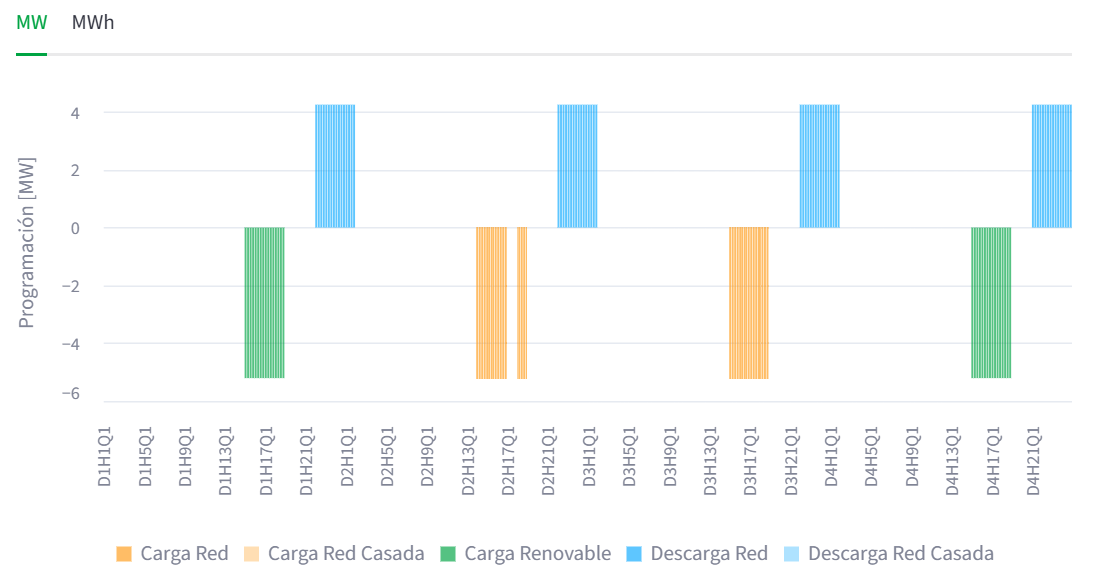
\includegraphics[width=0.75\linewidth]{figures/hibrida-flexible.png}
  \caption[Programa de la topología híbrida flexible.]{Programa de la topología híbrida flexible, en donde la batería es capaz de cargar de la generación como le convenga. Dado que existe recurso de generación, el sistema indica tomarlo para evitar peajes y costes asociados, excepto cuando la carga de la red negativa resulta más favorable.}%
  \label{fig:hibrida-flexible}
\end{figure}

\begin{figure}
  \centering
  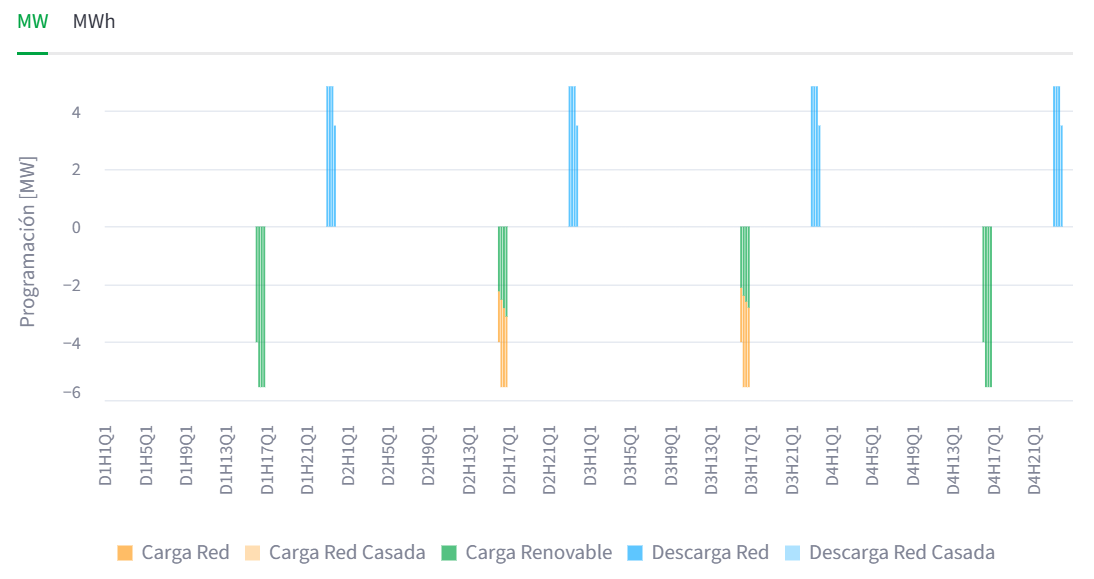
\includegraphics[width=0.75\linewidth]{figures/hibrida-prioridad.png}
  \caption[Programa de la topología híbrida con prioridad de carga de generación.]{ma de la topología híbrida con prioridad de carga de generación, en donde la batería no puede cargar hasta agotar el recurso de generación. Se observa como, aunque la batería quiera cargar de la red por la existencia de precios negativos beneficiosos, no es capaz de hacerlo.}%
  \label{fig:hibrida-prioridad}
\end{figure}

\begin{figure}
  \centering
  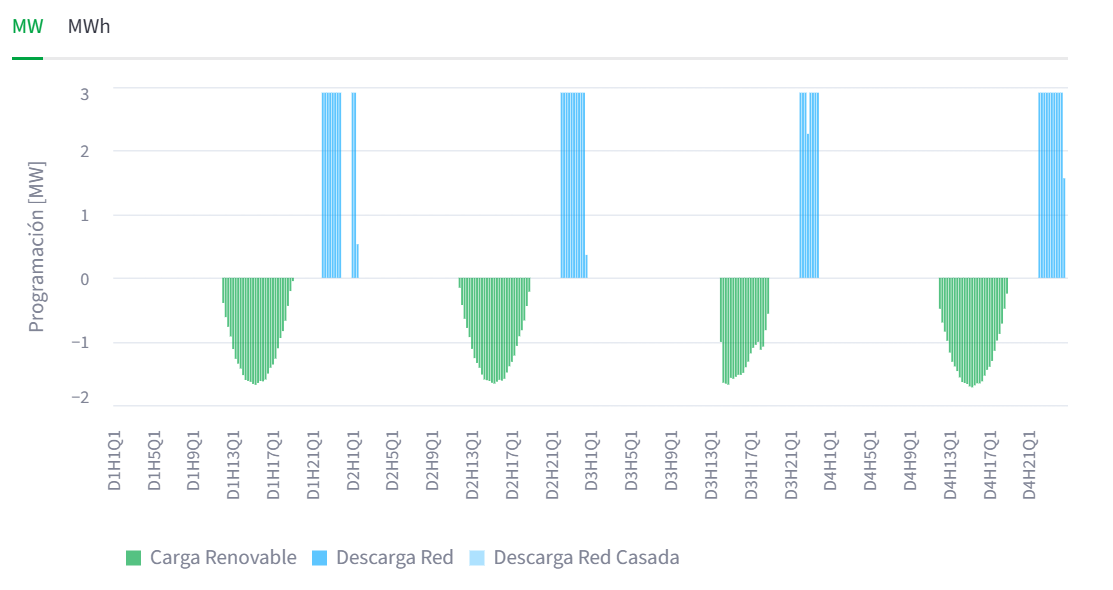
\includegraphics[width=0.75\linewidth]{figures/hibrida-aislada.png}
  \caption[Programa de la topología híbrida con carga aislada de la red.]{Programa de la topología híbrida con carga aislada de la red, en donde la batería solo en capaz de cargar cuando hay recurso de generación excedente. Como la carga es dependiente del recurso de generación, puede que la batería no sea capaz de ciclar completamente}%
  \label{fig:hibrida-aislada}
\end{figure}

En vista de los resultados obtenidos en la tabla~\ref{tab:comparacion-hibridacion}, la configuración híbrida flexible es la que mayor rentabilidad genera, ya que es capaz de cargar tanto de la red como de la generación energética. Una de las claves de su mejora de rendimiento resultan los precios de mercado negativos. Estos, muy comunes en periodos de baja demanda, permiten obtener beneficio por comprar o cargar energía con el propósito de mantener la estabilidad de la red.

La configuración híbrida con prioridad de carga de generación, en cambio, no permite el aprovechamiento de los precios negativos ya que, irónicamente, debe priorizar la carga híbrida precisamente en los periodos de mayor generación, los cuales se corresponden con los de menor precio. Es decir, la topología está perdiendo ingresos significativos por no poder cargar fácilmente durante precios negativos.

Por otro lado, la híbrida con carga aislada de la red es directamente incapaz de cargar de la red. Aunque con ella se asegure un \textit{lower bound} nulo del precio de compra, no se es capaz de aprovechar la generación al máximo debido a las restricciones de carga parcial de la generación, por lo que no realiza todos los ciclos asignados. También sucede una situación similar a la configuración topológica anterior en comparando el beneficio neto y por unidad de energía.

\begin{table}[ht]
  \centering
  \resizebox{\textwidth}{!}{%
    \begin{tabular}{|l|S|S|S|}
      \hline
      Configuración                                & {Beneficio [\si{\text{\euro}\per\mega\watt\hour}]} & {Beneficio [\si{\text{\euro}}]} & Ciclos \\
      \hline
      Híbrida flexible                             & 142.30                                             & 9562.90                         & 4.0    \\
      Híbrida con prioridad de carga de generación & 132.30                                             & 2567.10                         & 4.0    \\
      Híbrida con carga aislada de la red          & 126.90                                             & 2587.10                         & 2.3    \\
      \hline
    \end{tabular}
  }
  \caption[Comparación de configuraciones topológicas híbridas.]{Comparación de las métricas de las configuraciones topológicas híbridas.}%
  \label{tab:comparacion-hibridacion}
\end{table}

Se concluye que la configuración topológica flexible es esperadamente superior.

El integrador del sistema es capaz de modificar el funcionamiento físico \textit{on-site} de las instalaciones híbridas, incorporando el comportamiento flexible, para mejorar el rendimiento. Precisamente, tras el despliegue y obtención de resultados del sistema, la configuración topológica de una de las instalaciones se encuentra en proceso de modificación de híbrida con prioridad de carga de generación a híbrida flexible tras proponer el cambio.

\section{Arbitraje colaborativo}%
\label{makereference7.5}

Finalmente, aunque la operación automática del sistema sea superior al control manual, eso no significa que los agentes de mercado no deban modificar su operación si piensan que es necesario para aumentar el beneficio.

Los agentes de mercado que operan el cuadro de mandos del sistema son capaces de detectar patrones externos que escapan al sistema. Uno de los fenómenos correspondientes más claros resulta ser la influencia de la temporalidad.

La temporalidad se aprecia en los precios del mercado, variando drásticamente según la demanda energética. En épocas calurosas y frías el precio aumenta, al igual que a lo largo de la semana. Con esto, es posible estudiar dicha temporalidad para atinar el ratio de ciclado de la batería y aumentarlo en las épocas más favorables y disminuirlo en las menores.

\begin{figure}
  \centering
  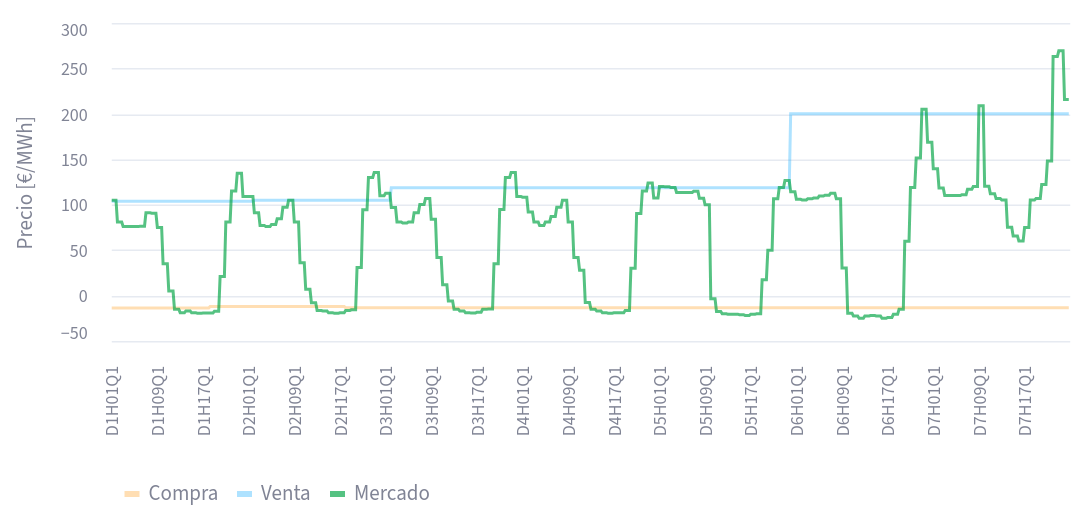
\includegraphics[width=0.75\linewidth]{figures/temporalidad-mercado.png}
  \caption[Variación del precio de mercado según el día de la semana.]{Variación del precio de mercado según el día de la semana.}%
  \label{fig:temporalidad-mercado}
\end{figure}

La figura~\ref{fig:temporalidad-mercado}, en la que se observa un pico enorme de \SI{269.39}{\text{\euro}\per\mega\watt\hour} a finales de la semana, muestra una diferencia de \SI{151.43}{\text{\euro}\per\mega\watt\hour} en la variación de los momentos oportunos de arbitraje\footnote{Curiosamente, el precio más alto de la historia es de \SI{544.98}{\text{\euro}\per\mega\watt\hour}~\cite{ecoavant2025precio}, aunque normalmente ronde los \SI{100.0}{\text{\euro}\per\mega\watt\hour} o menos}.

Un agente de mercado operando el cuadro de mandos del sistema, en cambio, puede conocer la temporalidad del mercado eléctrico y aprovechar los altibajos para indicarle al sistema un ritmo más alto o bajo del ciclado de las baterías.

Este modo de operación se conoce como arbitraje colaborativo y es recomendable para ajustar el comportamiento del sistema en busca del mayor beneficio, siendo, en consecuencia, el finalmente adoptado por la entidad de mercado.
